\title{INTD255, Safe Return Doubtful: Midterm 1}
\author{Dr. Jordan Hanson - Whittier College Dept. of Physics and Astronomy}
\date{\today}
\documentclass[10pt]{article}
\usepackage[margin=1.5cm]{geometry}
\usepackage{outlines}
\usepackage{graphicx}
\usepackage{amsmath}

\begin{document}
\maketitle

\section{Memory Bank}

\begin{itemize}
\item Acceleration due to gravity: $9 = 9.81$ m/s$^2$.
\item $T^2 = R^3$ ... Kepler's 3rd Law, if $T$ is the orbital period in years and $R$ is the orbital radius in AU.
\item $R_{AU} = D_E/\left(2\pi\Delta t (T_V^{-1} - T_E^{-1})\right)$
\item $W = F d$ ... Work (in Joules) is equal to force (in Newtons) times distance (in meters).
\item $f = \mu m g$ ... The force of friction if $f$ is in Newtons, $m$ is the mass in kilograms, and $g = 9.18$ m/s$^2$.  The number $\mu$ is called the coefficient of friction.
\item $W = \mu m g d$ ... Combining the above two formulas, we find the work in pulling a load against friction for some distance.
\item $W = mgh$ ... The work required to ascend a height $h$ carrying a mass $m$.
\item 1 kilocalorie, or 1 kcal, is equal to 4184 Joules.
\item The following conversions are useful: 1 gram of fat has 9 kcal of energy.  1 gram of protein has 4 kcal of energy.  1 gram of carbohydrate has 4 kcal of energy.
\item A distance \textit{vector} can be expressed as an amount of distance in a given direction.  We use the notation $\vec{x} = (a,b)$ to represent the amount of distance East ($a$), and the amount of distance North ($b$).
\item Vectors add like lists of numbers: $(a,b) + (x,y) = (a+x,b+y)$.
\item To calculate the \textit{length} of a vector $|\vec{x}|$, we use the Pythagorean theorem: $|\vec{x}| = \sqrt{a^2+b^2}$
\item To calculate the \textit{angle} $\theta$ a vector makes with the x-axis, we use trigonometry: $\theta = \tan^{-1}(b/a)$.
\end{itemize}

\section{The Planets}

\begin{enumerate}
\item Given the following planetary radii, calculate the orbital periods:
\begin{itemize}
\item Mercury: 0.387 AU
\item Venus: 0.723 AU
\item Mars: 1.524 AU
\end{itemize}
\item Given the following planetary orbital period, calculate the orbital radii:
\begin{itemize}
\item Jupiter: 11.862 years
\item Saturn: 29.457 years
\item Uranus: 80.02 years
\end{itemize}
\item There is a star named Tau Ceti that is only 12 light years away.  One of its planets, Tau Ceti e, has an orbital period of 163 days.  How far is it from the star, in AU?
\end{enumerate}

\section{Work, Force, and Friction}

\begin{enumerate}
\item Solve for the missing quantity:
\begin{itemize}
\item A) A man pulls a sled with a force of 100 N for 200 m.  How much work has he done?
\item B) A team of dogs pulls a sled, and each dog pulls with a force of 50 N.  The sled travels 5 km.  How much work is done by the team?
\item C) A man expends $10^5$ J pulling a sled, and he can pull with a force of 100 N.  How far did the sled go? 
\end{itemize} \vspace{3cm}
\item Suppose a sled that has 1500 kg of mass, and can be considered a system of waxed wood sliding on wet snow.  a) What would be the force of friction?  (Consult Tab. \ref{fig:friction} for the correct coefficient of friction).  b) If we pulled this sled for 10 km, how much energy would this require?  \vspace{2cm}
\begin{figure}[hb]
\centering
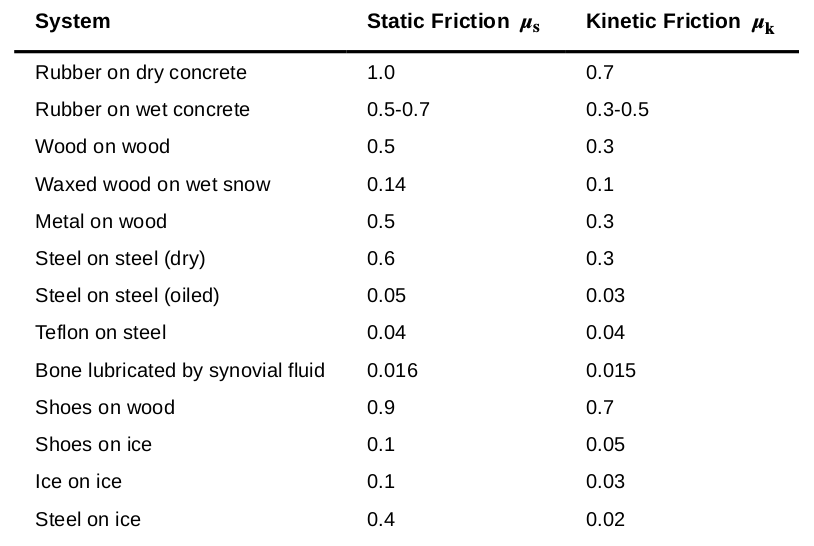
\includegraphics[width=0.45\textwidth]{friction.png}
\caption{\label{fig:friction} Frictional coefficients for different surfaces.}
\end{figure}
\end{enumerate}

\section{Food Energy and Unit Conversion}

\begin{enumerate}
\item Suppose we consume 75 grams of protein, 100 grams of carbohydrates, and 11 grams of fat.  How many kcal of energy did we gain? \\ \vspace{1cm}
\item a) Convert the energy in the previous problem from kcal to Joules.  b) Solve $W = \mu m g d$ for $d$, and assume the answer from part a) is $W$.  c) How far could we pull a 200 kg load with the energy gained from the food, if the frictional coefficient was 0.05? \\ \vspace{1cm}
\end{enumerate}

\section{Navigation}

\begin{enumerate}
\item Suppose a traveler heads South for 1 km, then West for 1 km, and rests.  The next day, the traveler heads Northwest (45 degrees above West) for 5 km.  a) Draw a graph of their path.  b) What is the final location?  c) How far are they from the origin? \\ \vspace{4cm}
\item Suppose a climber wants to climb straight upwards a vertical distance of 100 meters.  If he has a mass of 70 kg, how much energy does he need? \\ \vspace{2cm}
\end{enumerate}

\section{Summary}

\begin{enumerate}
\item Begin at the black diamond in Fig. \ref{fig:maze}.  Chart a course to the location of ARIANNA (white diamond). Assume a friction coefficient of 0.05 while on snow, and assume you are carrying 600 kg for the entire journey.  a) How much energy is required to get there? b) How much food would be required to achieve the goal?  (You can allocate different amounts of carbohydrates, protein, and fat, as long as it adds up to the number of kcal required). 
\begin{figure}[hb]
\centering
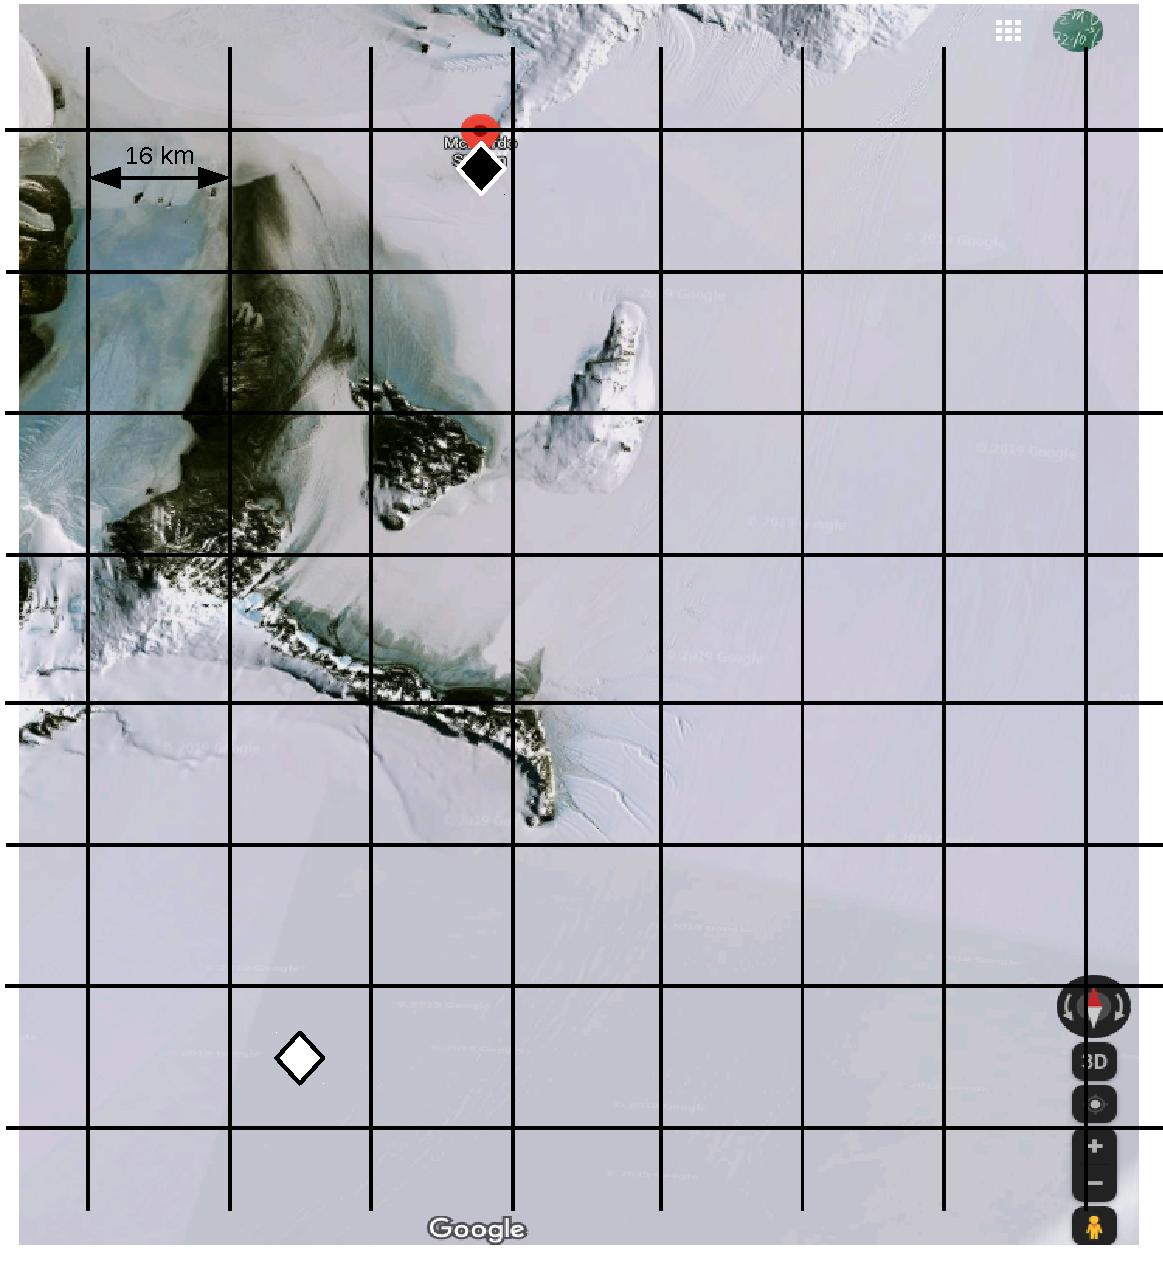
\includegraphics[width=0.5\textwidth]{glacier3.pdf}
\caption{\label{fig:maze} Map for the summary calculation.}
\end{figure}
\end{enumerate}

\end{document}
